\section{Literature}

The IPE literature on the relationship between politics and FDI has focused largely on how political factors shape and direct the flow of FDI across countries. Among the considered factors include: corruption, regime type, political violence, expropriation, etc. The dominant theoretical insight in this literature is the ``obsolescing bargain'' power of foreign firms. Once foreign firms sink their illiquid investment into the host countries, they no longer have a bargaining power and may be vulnerable to the caprice and avarice of the host. All of the political factors are a variant on what characteristics of the state mitigate or exacerbate this obsolescing bargaining problem.  Later analyses extend the framework to dyadic framework, examining the interplaying effect of both the host and the home country characteristics.

Is this interesting? Presumably it is interesting because we care about the role of the nation states in the international economy, which in turn it is important because the flow of FDI has welfare implications for millions of citizens in the host countries. A frequent policy conclusion from this body of research is echoed widely in the policy sphere is that countries need to improve the investment climate, reduce corruption, or maintain political stability to attract FDI.

But do countries want to? This causally prior question, and arguably more pregnant with politics, it has been understudied. 

On the one hand, some scholars have looked at the demand for FDI. However, these efforts have been stymied by recalcitrant issues with data and methods.

One the other hand, I also want to raise the issue of the quality of FDI.

Implicit in this phrase are two under-examined ideas: one is that country always want to attract FDI. Two is that it does not differentiate between the type of FDI that a country would want.

\subsection{Countries' demand for FDI}

Recognizing the need to theorize about the demand for FDI, scholars have recently paid more attention to this area \citep{Pinto2013, Pandya2016}. Similar to the rich IPE literature in trade and exchange rate \citep{Broz2001, Milner2005a}, these studies argue that countries' demand for FDI varies according to FDI's distributive effect on their domestic constituencies.\footnote{The alternative to preference as the explanan of FDI flow is institutional characteristics.} In this theoretical framework, labor supports FDI because foreign firms bring capital that increases the demand for labor and raises productivity, both of which lead to higher wage. On the other hand, domestic firms oppose FDI because foreign firms compete with them for labor, local inputs, and markets. Both \citet{Pinto2013} and \citet{Pandya2016} formulate their theories as a variant of this labor-vs-business tension, which surfaces in the former work as left-vs-right governments, and in the latter as democratic-vs-authoritarian regimes.

While these pioneering works have enriched our understanding of the relationship between politics and FDI, serious empirical issues prevent their statistical analyses from truly validating their theoretical arguments. The bottleneck is measuring country's demand for FDI.

For example, consider \citet{Pinto2008, Pinto2013}'s approach, which controls for economic and institutional factors that affect bilateral FDI flow into a country. The author then claims that the country's demand for FDI is what's left in the residual.\footnote{Specifically, the estimation of FDI openness involves two steps. First, the author runs a gravity model explaining bilateral FDI flows, estimating the intercept as the host country-year fixed effect. Second, this fixed effect is then regressed on several economic and endowment factors of that country-year (i.e. GDP, GDP per capita, average school years, arable land). The residual of the second stage is considered the country's ``FDI openness'' in that year.} For this approach to be valid, every economic, institutional, and endowment factors that affect FDI flow have to be controlled for, leaving only the country's demand in the error term. This claim is much stronger than the regular assumption of exogenous and normally distributed error, which is valid as long as the omitted factors are uncorrelated with the independent variable of interest. Framed substantively, since the residual is likely to contain more than just the country's demand for FDI, if we observe an abnormally high level of FDI we still do not know whether it is because the country welcomes FDI or because foreign firms find something attractive in the country.\footnote{In addition, the data requirement of bilateral FDI flows, ideally disaggregated by sectors, is very demanding. Therefore, this approach is limited to OECD countries only \citep{Pinto2008}. During the period the authors study, 1980-2000, OECD countries accounted for 95\% of global FDI outflow and 90\% of inflow. However, since then the role of the developed world in global FDI has declined sharply, reduced to 60.8\% of outflow and 40.6\% of inflow in 2014 \citep{UNCTAD2015}.}

In contrast to \citet{Pinto2013}'s statistical approach, \citet{Pandya2014, Pandya2016} aimed to substantively measure countries' demand for FDI, using the annual US Investment Climate Reports to code how many industries have foreign ownership restriction or face investment screening. This measurement is easier to interpret and available for many countries. However, two problems remain. First, adding up the raw count of restricted industries is not appropriate because industries are not all the same. For example, given the reach of the banking sector into all corners of the economy, a country's opening up its financial industry indicates much more FDI-friendliness than, say, allowing foreign furniture makers to set up shops. Since the theoretical argument is driven by FDI's distributive effect, it is suspect to ignoring the varying effect of FDI across sectoral constituencies. Second, given the coding rules, an industry is coded as free if there is no mention of restriction. If the industry in a FDI receives little FDI, it may not be worth mentioning, and yet still coded as open. Thus, where there is little FDI it may look like the country is extremely friendly. This concern is not hypothetical. \Cref{fig:china_fdi_restriction} shows that, following the coding of the US Investment Climate Reports, China seemed to be 100\% open to FDI up until 1986, when it started imposing restrictions. The reality is opposite. When China first opened up for FDI in 1979, only limited FDI is allowed as joint-venture in Special Economic Zones (SEZ). The year of 1986 was, in fact, the first time China allowed any wholly owned FDI outside of SEZs.

\begin{figure}[!ht]
\centering
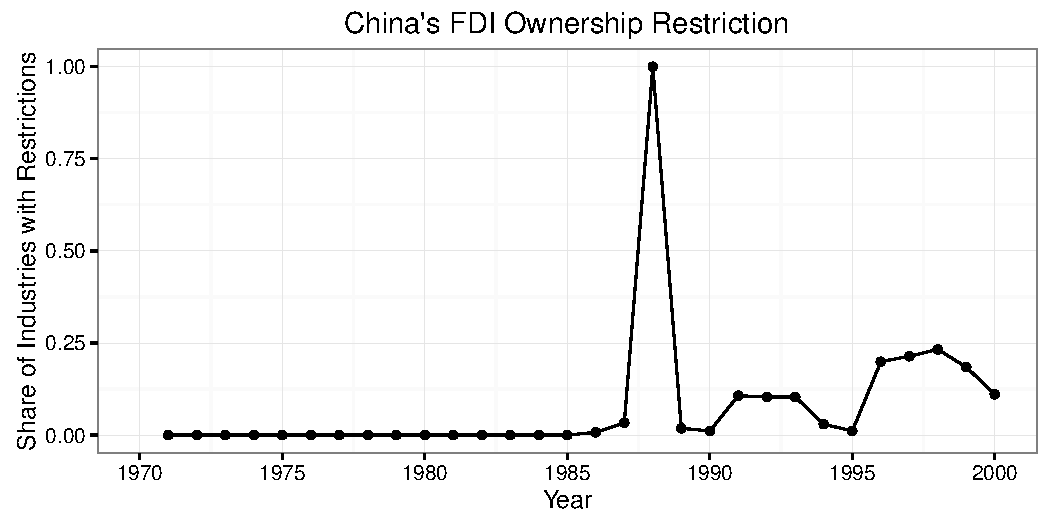
\includegraphics[width=0.75\textwidth,keepaspectratio]{../figure/china_fdi_restriction}
\caption{China's FDI Ownership Restriction, as coded in \citet{Pandya2010}. The sharp spike in 1988 also does not seem to correspond to any actual change in policy, and thus likely an artifact of reporting. See \citet{Zebregs2002} for a historical overview of China's FDI policy.}
\label{fig:china_fdi_restriction}
\end{figure}

\subsection{The measurement of FDI}

From Kerner, ``I suggest that most of what we claim requires FDI data does not. Instead, we are asking questions about employment, payrolls, capital inputs, and output from FDI. We should measure these instead.''

First is the aggregate nature of FDI data used by political science research.

FDI flow exclude locally raised finance data. This is appropriate for the purpose of measuring balance of payment, but not so much when we care about the actual size of the foreign firms in the country (808). The IMF has admitted to this problem, even suggesting in 2005 that FDI 
inflows data has become “
hardly applicable to sound economic analyses” 
due to this
(Ouddeken 2005)


FDI stock at market value fluctuates based on market price as well, something unrelated to the FDI firm behavior. FDI stock at historical value is simply the accumulation of FDI flow (as other countries calculate it).

Most of FDI literature has used FDI flow \citep{Jensen2003, Ahlquist2006, Beazer2011, Graham2010}. Some debate on measuring FDI, but it's on outliers and FDI or FDI/GDP \citep{Li2009}

Second, it allows us to get at the preferences of country. Previously, most of the research is on the preference of firms. Only two works by Pondya and Pablo Pinto looks at the other side.

The theoretical interest is there as scholars start to fill in the other side of the equation. However, the empirics left wanting.

All of these models also cannot investigate countries' preference for specific firms' characteristics. Pondya's look at cross industry, but because of data issue she can only do cross-sectional at the industry level instead of country-industry level. This level of aggregation is dubious: the same industry in one country is different from another country. For example, automobile value chain is vastly different across countries (example here)

All of the industry estimates are based on US firms, which really cannot be realized to others. (It can for some basic industry characteristics / technology level, not for whether an industry is market oriented or not.)

My data use capital size, which is great because that's exactly what countries look for. 


\citep[295]{Yamawaki1991} says that the data ``list virtually all the foreign subsidiaries of Japanese companies''